\documentclass[12pt, oneside, openany]{report}

%------------------------------------------------------------
% Language, encoding and line breaking
\usepackage[T1]{fontenc}
\usepackage[utf8]{inputenc}
\usepackage[english]{babel}
\usepackage{csquotes}
\usepackage{lmodern}
\usepackage{textcomp}
\usepackage{microtype}
\setlength{\emergencystretch}{3em}
%------------------------------------------------------------
% Page layout and general packages
\usepackage{graphicx}
\usepackage[table]{xcolor}
\usepackage[left=3.00cm, right=3.00cm, top=2.50cm, bottom=2.50cm]{geometry}
\usepackage{makecell}
\usepackage{ragged2e}
\usepackage{indentfirst}
\usepackage{fancyhdr}
\setlength{\headheight}{29.2pt}
\addtolength{\topmargin}{-17.2pt}
\usepackage{tabularx}
\usepackage{array}
\usepackage{booktabs}
\usepackage{adjustbox}
\usepackage{float}
\usepackage{enumitem}
\usepackage{siunitx}
\sisetup{detect-all}
\usepackage{amsmath, amssymb, amsfonts}
\usepackage[tablewithin=none,figurewithin=none]{caption}
%------------------------------------------------------------
% TikZ diagrams
\usepackage{tikz}
\usetikzlibrary{positioning,arrows.meta,shapes.geometric,calc}
%------------------------------------------------------------
% Bibliography (numeric citations, run with biber)
\usepackage[style=numeric-comp, sorting=none, backend=biber]{biblatex}
\addbibresource{bib.bib}
%------------------------------------------------------------
% Colors (NASA Space Apps palette)
\definecolor{spaceBlue}{RGB}{7, 23, 63}
\definecolor{electricBlue}{RGB}{0, 66, 166}
\definecolor{rocketRed}{RGB}{226, 78, 66}
\definecolor{softGray}{RGB}{235, 239, 245}
%------------------------------------------------------------
\usepackage{xurl}
\usepackage[hidelinks]{hyperref}
\usepackage{titlesec}
\titleformat{\chapter}[display]{\huge\scshape\color{spaceBlue}}{\textbf{\chaptername~\thechapter}}{12pt}{}
\titleformat{\section}{\Large\bfseries\color{electricBlue}}{\thesection}{1em}{}
\setlength{\parindent}{12pt}
%------------------------------------------------------------
% Screenshot helper: includes Figuras/<name>.png (or .jpg) if present,
% otherwise draws a framed placeholder so the document always compiles.
\newcommand{\screenshot}[2]{%
  \IfFileExists{Figuras/#1.png}{\includegraphics[width=#2\linewidth]{Figuras/#1.png}}{%
  \IfFileExists{Figuras/#1.jpg}{\includegraphics[width=#2\linewidth]{Figuras/#1.jpg}}{%
    \fbox{\parbox[c][5cm][c]{#2\linewidth}{\centering\color{gray}\small
      Screenshot placeholder\\[2pt]\texttt{Figuras/#1.png}}}}}}
%------------------------------------------------------------
% Short-hands
\newcommand{\EarthScope}{\textsc{EarthScope}}
\newcommand{\perdecade}{\,per decade}

\title{EarthScope: Hidden Climate Signals}
\author{Team astro-burritos}
\date{November 2026}

\begin{document}
\pagestyle{empty}

%------------------------------------------------------------
%    COVER
%------------------------------------------------------------
\begin{center}
    {\large\color{electricBlue} NASA Space Apps Challenge 2026}\\[4pt]
    {\normalsize Challenge: \enquote{Be an Earth System Trend Detective!}}

    \vspace*{2.2cm}
    {\large Technical Report}\\[0.6cm]
    {\Huge\bfseries\color{spaceBlue} EarthScope}\\[0.3cm]
    {\LARGE Hidden Climate Signals}\\[0.5cm]
    {\large\itshape Which climate signals are changing,\\ and can we trust them?}

    \vspace*{2.2cm}
    Presented by:\\[4pt]
    \textbf{Team astro-burritos}\\[6pt]
    % Team members, in alphabetical order by surname
    \textbf{Jayme Said Barbosa Hernández}\\
    \textbf{Guillermo Carreto Sánchez}\\
    \textbf{Juan Carlos Flores Mora}\\
    \textbf{Samuel Soriano Chávez}

    \vspace*{1.6cm}
    Live application: \url{https://earthscope-chi.vercel.app}
\end{center}

\vfill
\raggedleft{November \textbf{2026}}

\vspace{0.8cm}
\begin{center}
    \textcolor{rocketRed}{\rule{12cm}{0.8mm}}\\[4pt]
    \small\textit{EarthScope is an independent Space Apps project. It is not an official NASA product, and NASA does not endorse it.}
\end{center}
\justify

%------------------------------------------------------------
%    FRONT MATTER
%------------------------------------------------------------
\clearpage
\setcounter{page}{1}
\pagenumbering{roman}
\pagestyle{plain}

\chapter*{High-Level Summary}
\addcontentsline{toc}{chapter}{High-Level Summary}

\noindent\textbf{Project name:} EarthScope -- Hidden Climate Signals

\vspace{0.3cm}
% Space Apps requirement: 50-200 words (this summary: ~170 words)
We developed \EarthScope{}, a free web application that finds long-term climate trends in NASA data for almost any place on Earth and shows the statistical evidence behind each one. A user picks a country or state on a 3D globe, a period and one of 13 climate variables, and presses \emph{Analyze}. The server requests live data from the NASA POWER API (MERRA-2) and returns the trend per decade with its 95\% interval, an autocorrelation-corrected test, five robustness checks and the smallest trend the data could detect. It answers the challenge's four questions---what is changing, where, how much and whether it is significant---and only says \enquote{increase} or \enquote{decrease} when the evidence supports it. A second NASA rain record (GPM IMERG) and a second place cross-check every result, and an exploratory projection appears only if it beats the historical mean on held-out years. This matters because local climate decisions need evidence people can trust: \EarthScope{} makes NASA data accessible without overstating what it shows. For example, mean temperature in Puebla, Mexico, rose \SI{+0.45}{\celsius}\perdecade{} (2001--2024), passing all five checks.

\vspace{0.4cm}
\noindent\textbf{Keywords:} climate trends, NASA POWER, MERRA-2, GPM IMERG, Mann--Kendall, robustness, science communication, open data.

\section*{Project demo and project links}

\begin{itemize}[leftmargin=*]
    \item \textbf{Project demo (30-second video, English captions):} \url{[DEMO VIDEO LINK]}
    \item \textbf{Project (live application):} \url{https://earthscope-chi.vercel.app}
    \item \textbf{Source code:} \url{https://github.com/Jimbotz/astro-burritos}
\end{itemize}

\noindent All links are public and require no password, permission or registration. The demo contains no names, voices or likenesses of anyone under the age of 18.

\tableofcontents

%------------------------------------------------------------
%    CONTENT
%------------------------------------------------------------
\clearpage
\pagenumbering{arabic}
\setcounter{page}{1}
\pagestyle{fancy}
\fancyhf{}
\fancyhead[R]{\small\rightmark}
\fancyfoot[C]{\thepage}

%============================================================
\chapter{Introduction}
%============================================================

Climate change is usually communicated through global numbers: the planet has warmed by about one degree, sea level is rising, extremes are more frequent. People, however, make decisions locally. A farmer in central Mexico, a municipal planner or a teacher wants to know what has changed \emph{where they live}, by how much, and whether that change is real or just year-to-year noise.

NASA already offers the raw material to answer those questions. The NASA POWER project \cite{nasapower} serves more than four decades of daily and monthly climate variables for any coordinate on Earth through a free, keyless API, derived from the MERRA-2 reanalysis \cite{gelaro2017merra2}. The Global Precipitation Measurement mission provides an independent, satellite-based rain record (IMERG) \cite{huffman2020imerg}. What is missing is the step between a column of numbers and a statement that a non-specialist can trust.

The NASA Space Apps Challenge 2026 challenge \enquote{Be an Earth System Trend Detective!} \cite{spaceapps2026} asks participants to close that gap: to use NASA Earth data to discover \emph{what} is changing, \emph{where}, \emph{how much}, and whether the change is \emph{significant}. Team astro-burritos answered with \EarthScope{}, a public web application that pairs every trend with the statistical evidence behind it and refuses to make claims that the data cannot support.

This report presents the project. Chapter~\ref{cap:problem} describes the problem and why the challenge matters. Chapter~\ref{cap:solution} shows what \EarthScope{} does from the user's point of view, and Chapter~\ref{cap:data} lists where the data come from. Chapter~\ref{cap:how} explains only the technical aspects that make the results trustworthy: the trend tests, the charts and the exploratory projection. Chapter~\ref{cap:relevance} discusses relevance and limitations, Chapter~\ref{cap:ai} explains how artificial intelligence was used responsibly during development, and Chapter~\ref{cap:conclusions} concludes.

%============================================================
\chapter{Problem and justification}\label{cap:problem}
%============================================================

\section{The problem}

Open climate data are abundant, but using them correctly is hard. Four obstacles stand between NASA's archives and a trustworthy local answer:

\begin{enumerate}[leftmargin=*]
    \item \textbf{Access and format.} Data are served as gridded fields, parameter codes (\texttt{T2M}, \texttt{PRECTOTCORR}, \ldots) and fill values. Choosing the right variable, endpoint, time standard and aggregation already requires expertise.
    \item \textbf{Naive statistics overstate change.} Climate series are short and autocorrelated: a warm year tends to follow a warm year. A plain least-squares line or a textbook Mann--Kendall test treats each year as independent and therefore reports \enquote{significant} trends far too often \cite{hamed1998,yue2002tfpw}.
    \item \textbf{Many tests, many false alarms.} Looking at 13 variables, or at dozens of grid cells on a map, guarantees that some will look significant by chance unless the multiple comparisons are controlled \cite{bh1995,wilks2016}.
    \item \textbf{Absence of evidence is read as evidence of absence.} When a test finds nothing in 24 years of data, the honest conclusion is \enquote{these data cannot detect a trend of this size}, not \enquote{nothing has changed}.
\end{enumerate}

Added to these is a support problem: a reanalysis value represents a grid cell of roughly \SI{55}{\km} $\times$ \SI{65}{\km} with its own mean elevation, not a city or a weather station. Presenting it as \enquote{the temperature of Puebla} is misleading.

The result is a gap with two failure modes. Either the data stay unused because they are too hard to handle, or they are used carelessly and produce confident claims that do not hold up.

\section{Why the challenge is relevant}

Local climate evidence matters for concrete decisions: which crops and planting dates to choose, how to size water storage, when to expect heat stress, how to prioritise public health warnings. In central Mexico, for example, warmer nights affect crops and human health, and rain variability drives agricultural risk. Communities in regions with few weather stations have no other long, consistent record than satellite and reanalysis products.

At the same time, public trust in climate science depends on claims being right. An application that exaggerates a trend---or that reports a rain trend that a second independent dataset contradicts---damages that trust. The challenge is therefore relevant on two levels: it democratises NASA data, and it asks for tools that teach users to separate signal from noise.

\section{Objectives}

\subsection*{General objective}
Build a public web application that lets anyone detect long-term climate trends in NASA data for almost any place on Earth and judge how much each result can be trusted.

\subsection*{Specific objectives}
\begin{enumerate}[leftmargin=*]
    \item Retrieve NASA POWER data live, with no accounts or keys, for any country or state selected on an interactive globe.
    \item Report each trend as a rate per decade with its 95\% interval, an autocorrelation-corrected $p$-value and the minimum detectable trend.
    \item Allow the words \enquote{increase} or \enquote{decrease} only when a trend passes pre-declared robustness criteria.
    \item Show the spatial pattern on a map of native grid cells, with field-wise control of false discoveries.
    \item Cross-check results against a second NASA rain record and a second place.
    \item Offer an exploratory projection only when it passes an out-of-sample skill test, always with its uncertainty.
\end{enumerate}

%============================================================
\chapter{The solution: EarthScope}\label{cap:solution}
%============================================================

\EarthScope{} \cite{earthscope} is a single-page web application. Its guiding principle is that \emph{claims are earned}: every number comes from NASA at request time, and the strength of the wording follows the strength of the evidence.

\section{What it answers}

Table~\ref{tab:questions} maps the four questions of the challenge to what \EarthScope{} shows.

\begin{table}[H]
\centering
\caption{The challenge's four questions and how EarthScope answers them.}
\label{tab:questions}
\begin{tabularx}{\linewidth}{@{}lX@{}}
\toprule
\textbf{Question} & \textbf{How EarthScope answers it} \\
\midrule
\textbf{What} is changing? & 13 processed variables from NASA POWER: mean, maximum and minimum temperature, diurnal range, hottest day and coldest night of the year, warm days and warm nights, annual and wet-season rain, specific and relative humidity, and root-zone soil wetness. \\
\textbf{Where}? & Any country or state, selected on a 3D globe, plus a 2D map of native NASA POWER cells (\ang{0.5} $\times$ \ang{0.625}). \\
\textbf{How much}? & A rate per decade with its 95\% interval, and the smallest trend these years of data could detect. \\
\textbf{Is it significant}? & Five robustness checks before any \enquote{increase} or \enquote{decrease} appears; a second NASA rain record and a second place cross-check the result. \\
\bottomrule
\end{tabularx}
\end{table}

\section{How a user works with it}

\begin{enumerate}[leftmargin=*]
    \item \textbf{Pick a place and a variable.} The user chooses a country or state on the globe (Figure~\ref{fig:globe}) or in the autocomplete lists, a period (2001--2024 by default), a variable and a map layer. Nothing is downloaded until the user presses \emph{Analyze}.
    \item \textbf{Read the result.} The server returns a plain-language headline, the annual series (incomplete years are drawn as gaps, never as zero), the trend with its verdict---\emph{robust}, \emph{probable}, \emph{weak} or \emph{no trend detectable}---seasonal sub-series and an \emph{evidence file} with every test and the exact NASA request (Figure~\ref{fig:result}).
    \item \textbf{See it on the map.} Every native cell inside the state is colored by recent anomaly, trend per decade or average. Cells whose trend is significant across the whole field are outlined (Figure~\ref{fig:map}).
    \item \textbf{Cross-check.} Two cards ask whether the result holds up: \emph{Two NASA rain records} compares MERRA-2 with GPM IMERG for the same cell, and \emph{Two places, same rules} repeats the analysis at a second location.
    \item \textbf{Explore a projection.} For four variables, a straight line per cell is animated ten years past the data, labelled \enquote{exploratory, not a forecast} and always drawn with its 95\% prediction interval.
\end{enumerate}

The URL stores the whole query, so any result can be shared as a link.

\begin{figure}[H]
    \centering
    \screenshot{globe}{0.85}
    \caption{The 3D globe used to select a country or state.}
    \label{fig:globe}
\end{figure}

\section{The charts EarthScope generates, explained}

All the figures in this section are real captures of the application analysing Puebla, Mexico (cell centred at \ang{19.00}\,N, \ang{98.125}\,W, mean elevation \SI{2147}{\m}) for 2001--2024 with live NASA POWER data. Every chart is generated from the numbers returned at request time; none is a stored image.

\subsection{Result headline and statistical summary}

\begin{figure}[H]
    \centering
    \screenshot{result-puebla}{0.95}
    \caption{Result for Puebla, mean air temperature (2 m), 2001--2024: headline, spatial and temporal scope, statistical summary and the start of the annual series.}
    \label{fig:result}
\end{figure}

Figure~\ref{fig:result} is the first thing a user reads after pressing \emph{Analyze}. The green headline states the finding in one sentence---mean air temperature rose \SI{+0.45}{\celsius}\perdecade, \enquote{a robust trend that passes all five checks}---and immediately names the spatial support: a NASA POWER cell of \ang{0.5} $\times$ \ang{0.625} with its mean elevation, not a city value. The \emph{Spatial \& temporal scope} block reports the returned coverage (1981--2024) and how many incomplete years were excluded (none). The \emph{Statistical summary} lists the evidence line by line: the OLS trend (\SI{+0.45}{\celsius}\perdecade), its 95\% confidence interval (\num{+0.23} to \num{+0.70}), the Hamed--Rao $p$-value (0.0092), the $q$-value after correcting for the 13 variables tested (0.0299), the plain Mann--Kendall $p$-value, the 24 complete years used and the robustness score (5/5). Each underlined term opens a plain-language explanation.

\subsection{Historical observations and key signals}

\begin{figure}[H]
    \centering
    \screenshot{result-tnn}{0.95}
    \caption{Coldest night of the year (TNn) in Puebla: statistical summary, annual series with its Sen trend line, and the four robust signals of the cell.}
    \label{fig:result-tnn}
\end{figure}

Figure~\ref{fig:result-tnn} shows the same layout for the coldest night of the year. The \emph{Historical observations} chart plots one point per year (blue line) and the trend over complete years (dashed red line). The vertical axis is scaled to the data range ($-0.45$ to \SI{4.49}{\celsius}), and a missing year would appear as a gap, never as a zero. The badge \enquote{\SI{+1.64}{\celsius}, 2024 vs 2001} gives the raw change, and \emph{Export CSV} downloads the plotted values. Because TNn is one extreme value per year, its profile uses the robust Sen slope (\SI{+1.10}{\celsius}\perdecade, interval \num{+0.38} to \num{+1.92}) instead of OLS. The caption under the chart reminds the reader that \enquote{a trend does not establish causation}. On the right, \emph{Key signals at this cell} ranks the four variables with a robust trend: mean daily minimum temperature (\SI{+0.52}{\celsius}\perdecade), mean air temperature (\SI{+0.45}{\celsius}), coldest night (\SI{+1.10}{\celsius}) and warm nights (\num{+5.5} percentage points\perdecade). Warming at night is the clearest signal in Puebla.

\subsection{All climate signals: series, climatology and checks}

\begin{figure}[H]
    \centering
    \screenshot{signals-temperature}{0.95}
    \caption{\enquote{All climate signals} panel, temperature tab: annual series, 1991--2020 monthly climatology, change per decade with the five checks, and one card per variable.}
    \label{fig:signals-temp}
\end{figure}

The \emph{All climate signals} panel (Figure~\ref{fig:signals-temp}) puts the 13 variables side by side. The cards on the right show each variable's change per decade and its verdict badge; only \emph{Robust trend} cards get a green arrow. For example, mean daily maximum temperature (\SI{+0.37}{\celsius}\perdecade) and the hottest day (\SI{+0.05}{\celsius}) read \enquote{No detectable trend}, so they carry no arrow even though their numbers are positive. Selecting a card redraws the left side:
\begin{itemize}[leftmargin=*]
    \item the \textbf{annual series} with its trend line, switchable between values and anomalies against 1991--2020;
    \item the \textbf{1991--2020 monthly climatology}, the average seasonal cycle of the variable at this cell (here, coldest nights between \num{2.36} and \SI{10.26}{\celsius}, warmest from May to August);
    \item the \textbf{change per decade} with its likely range, and the \textbf{five checks} written in plain language: still significant with 13 variables tested at once; likely range excludes zero; holds after removing year-to-year memory; holds when any single year is dropped; same direction over 1981--2024.
\end{itemize}

\begin{figure}[H]
    \centering
    \screenshot{signals-rain}{0.95}
    \caption{Precipitation tab: rain variables are shown with their numbers but with \enquote{No trend claim}.}
    \label{fig:signals-rain}
\end{figure}

The precipitation tab (Figure~\ref{fig:signals-rain}) shows the \emph{show without claim} policy. Annual precipitation is \num{+7.3}\% per decade (\enquote{Weak signal}) and wet-season rain \num{+4.1}\% per decade (\enquote{No detectable trend}), and both carry the extra label \enquote{No trend claim}. Because POWER rain barely follows year-to-year changes at the stations, \EarthScope{} never turns a rain number into an \enquote{increase} or \enquote{decrease}.

\begin{figure}[H]
    \centering
    \screenshot{all-signals}{0.95}
    \caption{Humidity tab: specific humidity is a \enquote{Weak signal} and relative humidity has \enquote{No detectable trend}; neither gets an arrow.}
    \label{fig:signals}
\end{figure}

Figure~\ref{fig:signals} shows the two weakest levels of evidence. Specific humidity rises \SI{+0.30}{\g\per\kg}\perdecade{} with an interval that excludes zero, but it does not pass enough checks, so it is only a \enquote{Weak signal}. Relative humidity (\num{+0.4} percentage points\perdecade, interval $-1.1$ to $+1.9$) is \enquote{No detectable trend}, which is not the same as \enquote{no change}.

\subsection{Map of native cells}

\begin{figure}[H]
    \centering
    \screenshot{map-anomaly}{0.95}
    \caption{Globe and 2D map of Puebla: the 21 native NASA POWER cells colored by the recent anomaly of the coldest night (2020--2024 vs 1991--2020).}
    \label{fig:map-anomaly}
\end{figure}

The map (Figure~\ref{fig:map-anomaly}) clips the native POWER grid to the state outline and draws each cell as a raw rectangle, with no smoothing. In this layer each cell is colored by its recent anomaly: how much warmer (red) or colder (blue) its 2020--2024 average is than its 1991--2020 average. The diverging scale is centered on zero and symmetric ($\pm$\SI{2.37}{\celsius}), saturating at the 95th percentile so that one extreme cell does not wash out the others. The yellow dot marks the analysis point, and a \SI{100}{\km} scale bar gives the size. Most of Puebla is warmer than its baseline, more strongly in the south-west.

\subsection{The two cross-check cards}

\begin{figure}[H]
    \centering
    \screenshot{crosscheck}{0.95}
    \caption{Cross-check cards for Puebla: two NASA rain records (left) and two places with the same rules (right).}
    \label{fig:crosscheck}
\end{figure}

The left card in Figure~\ref{fig:crosscheck} overlays the annual rain of MERRA-2 (blue) and GPM IMERG (purple) for the same cell, each with its dashed trend line, and answers three questions:
\begin{enumerate}[leftmargin=*]
    \item \textbf{Same amount of rain? Yes.} MERRA-2 gives \SI{884}{\mm} and IMERG \SI{913}{\mm} a year on average, within the $\pm10\%$ rule.
    \item \textbf{Same wet and dry years? Yes, partly.} After removing each record's own trend, their correlation is $r = 0.68$.
    \item \textbf{Same trend? Not settled.} Neither record detects a trend: MERRA-2 has Hamed--Rao $p = 0.05005$, just above the 0.05 limit, and IMERG has $p = 0.5030$.
\end{enumerate}
The verdict is therefore \emph{Inconclusive}, and the card explains why the result should or should not be trusted: the two records are built differently but are only partly independent, and this period crosses the 2014 TRMM-to-GPM transition. (In Tlaxcala the same card returns \emph{Disagree}; see the examples below.)

The right card repeats the coldest-night analysis in Tehuacán with the same tests. Puebla has a robust trend of \SI{+1.10}{\celsius}\perdecade{}, whereas Tehuacán shows \SI{+0.30}{\celsius}\perdecade{} with an interval that includes zero ($-0.57$ to $+1.28$), so it is \enquote{No detectable trend}. The chart overlays both series, and the conclusion is stated carefully: \enquote{Only Puebla has a detectable trend. The record of Tehuacán can neither confirm nor rule out the same change.}

\subsection{Exploratory projection: when it runs and when it is blocked}

\begin{figure}[H]
    \centering
    \screenshot{area-map}{0.95}
    \caption{Exploratory projection of mean air temperature in Puebla: each cell is shaded by its fitted line, hatched cells are not significant across the field, and the warnings appear under the slider.}
    \label{fig:map}
\end{figure}

\begin{figure}[H]
    \centering
    \screenshot{projection-blocked}{0.95}
    \caption{Projection of the coldest night blocked by the quality test, with the regional series of Puebla's 21 cells below.}
    \label{fig:projection-blocked}
\end{figure}

Figures~\ref{fig:map} and~\ref{fig:projection-blocked} show both outcomes of the projection's quality test. For mean air temperature (Figure~\ref{fig:map}) the line passed the test, so the map animates 2001--2034: each cell darkens as its line rises. The panel reports that lines rise in all 21 cells (19 with a significant trend) and that two hatched cells are not significant across the field. It also lists the warnings: in 2015--2019 the line predicted worse than the average, only 70\% of held-out years fell inside the 95\% interval (at least 80\% expected), and the regional series bends upward.

For the coldest night (Figure~\ref{fig:projection-blocked}) the projection is \emph{blocked by quality}. On the held-out years 2015--2024 the line beats the average by only 4\% (the minimum is 10\%): $-0\%$ in 2015--2019 and $+8\%$ in 2020--2024. Nothing is extrapolated, and the map keeps showing the measured data. Below it, the \emph{Data layer} chart shows the area-weighted regional series of the 21 cells (\SI{+0.79}{\celsius}\perdecade, \enquote{Probable trend}). It is labelled as the regional mean of each cell's coldest night, not the coldest night in the region.

\subsection{Evidence file}

\begin{figure}[H]
    \centering
    \screenshot{evidence}{0.95}
    \caption{Evidence file: data source, retrieval time, API version, method and warnings for the selected variable.}
    \label{fig:evidence}
\end{figure}

Every result ends with an \emph{Evidence file} (Figure~\ref{fig:evidence}). It states the exact NASA product (NASA POWER, \texttt{T2M\_MIN}, monthly records, annual minimum), when it was retrieved, the source model and API version (MERRA-2, POWER API v2.10.0, local solar time), and a direct link to the NASA POWER request so anyone can download the same numbers. It also gives the method (Sen slope with a Gilbert interval and Hamed--Rao $p$-value), the verdict, the analysis warnings (\enquote{a single day per year: noisier than the mean minimum}) and the status \enquote{descriptive, source-linked}. Above it, the rain card shows the minimum detectable trend: a trend would need to be about \SI{107}{\mm}\perdecade{} (MERRA-2) or \SI{143}{\mm}\perdecade{} (IMERG) to be detectable in this cell.

\section{What it found: four examples}

The following results are reproducible with one click from the \emph{Try an example} buttons of the application.

\begin{enumerate}[leftmargin=*]
    \item \textbf{Warming that passes every test.} In Puebla, Mexico, over 2001--2024, mean air temperature rose \SI{+0.45}{\celsius}\perdecade{} (95\% interval \num{+0.23} to \num{+0.70}; Hamed--Rao $p = 0.009$), and warm nights rose 5.5 percentage points\perdecade. Both pass all five robustness checks.
    \item \textbf{The same signal in a second place.} Tehuacán, about \SI{110}{\km} to the southeast, shows the same signal for mean temperature (\SI{+0.62}{\celsius}\perdecade). Warm days (TX90p) rise detectably in Tehuacán but not in Puebla: part of the signal is shared and part is local.
    \item \textbf{Two NASA records disagree on rain.} In Tlaxcala, the MERRA-2 rain record alone shows a rise of \SI{+185}{\mm}\perdecade{} ($p < 0.001$). The satellite-based GPM IMERG record of the same cell shows \SI{-27}{\mm}\perdecade{} (not significant), and their 95\% intervals do not overlap. \EarthScope{} labels this \emph{Disagree} and makes no rain claim.
    \item \textbf{\enquote{No trend detected} is not \enquote{no change}.} When a test finds nothing, \EarthScope{} shows how large a trend would have to be before these years could detect it. In Puebla, a rain trend would need to be about \SI{107}{\mm}\perdecade{} in MERRA-2 to be detectable (Figure~\ref{fig:evidence}).
\end{enumerate}

%============================================================
\chapter{Data sources}\label{cap:data}
%============================================================

Every source used by the application is public and requires no login, key or token. Each response records the exact NASA requests it used, and the evidence file links to them, so any number can be traced back to its origin. Table~\ref{tab:sources} summarises the sources.

\begin{table}[H]
\centering
\caption{Data sources used by EarthScope.}
\label{tab:sources}
\small
\begin{tabularx}{\linewidth}{@{}>{\raggedright\arraybackslash}p{3.3cm}>{\raggedright\arraybackslash}p{3.6cm}X@{}}
\toprule
\textbf{Source} & \textbf{Product and resolution} & \textbf{Use in EarthScope} \\
\midrule
NASA POWER API v2.10 \cite{nasapower} & MERRA-2 reanalysis \cite{gelaro2017merra2}; monthly, daily and regional endpoints; native cell \ang{0.5} $\times$ \ang{0.625}; from 1981 & Every variable, the map grid and the projection (live) \\
NASA POWER API v2.10 & GPM IMERG monthly precipitation \cite{huffman2020imerg} (\texttt{IMERG\_PRECTOT}); \ang{0.1} pixels, UTC only, from 1998 & Second rain record of the cross-check card (live) \\
NOAA GHCN-Daily \cite{ghcnd} & Station records: Puebla airport and Tlaxcala & Offline validation only \\
Natural Earth \cite{naturalearth} & Countries 1:50m, states 1:10m; public domain & Globe outlines, selectors, 2D map, server-side area lookup \\
NASA Blue Marble \cite{bluemarble} & Global true-color Earth imagery & Globe texture (visual only, never data) \\
\bottomrule
\end{tabularx}
\end{table}

\section{NASA data used, with links}

\begin{itemize}[leftmargin=*]
    \item \textbf{NASA POWER} (Prediction Of Worldwide Energy Resources), NASA Langley Research Center, the challenge's resource and the source of every value: \url{https://power.larc.nasa.gov/}
    \item NASA POWER API documentation (temporal endpoints used: \texttt{monthly/point}, \texttt{daily/point}, \texttt{monthly/regional}): \url{https://power.larc.nasa.gov/docs/services/api/}
    \item \textbf{MERRA-2} reanalysis, NASA Global Modeling and Assimilation Office (the model behind POWER's climate variables): \url{https://gmao.gsfc.nasa.gov/gmao-products/merra-2/}
    \item \textbf{GPM IMERG} monthly precipitation, NASA Global Precipitation Measurement mission (served through POWER as \texttt{IMERG\_PRECTOT}): \url{https://gpm.nasa.gov/data/imerg}
    \item \textbf{NASA Blue Marble}, NASA Earth Observatory (globe texture): \url{https://science.nasa.gov/earth/earth-observatory/collections/blue-marble/}
\end{itemize}

\noindent A reproducible request for the Puebla cell, the same one the application sends:

\begin{center}
\footnotesize
\begin{minipage}{0.95\linewidth}
\raggedright\ttfamily
https://power.larc.nasa.gov/api/temporal/monthly/point?parameters=T2M,T2M\_RANGE, T2M\_MAX,T2M\_MIN,PRECTOTCORR,QV2M,RH2M,GWETROOT\&community=AG \&longitude=-98.2\&latitude=19.04\&start=1981\&end=2024\&format=JSON \&time-standard=LST
\end{minipage}
\end{center}

\section{NASA POWER and MERRA-2}

The core data source is the NASA POWER project of NASA Langley Research Center. Its \texttt{monthly/point} and \texttt{daily/point} endpoints return the nearest native MERRA-2 cell for a coordinate, together with its mean elevation; \EarthScope{} always labels values as belonging to that cell, never to a city or station. The \texttt{monthly/regional} endpoint feeds the map, requested in aligned \ang{5} tiles. Point series always start in 1981 so that the 1991--2020 climate baseline used for anomalies is complete.

An audit of POWER's variables preceded the choice of the 13 that the application processes. Seventeen more were evaluated and excluded, for reasons such as product changes in cloud and radiation records, non-homogenised wind and pressure, or unreliable daily rain indices. Each exclusion and its reason is recorded in the variable catalog of the code.

\section{GPM IMERG through POWER}

To test the rain record, \EarthScope{} uses GPM IMERG, a satellite-based precipitation product, through the same POWER API, which avoids the Earthdata login that other NASA portals require. IMERG is available only in UTC and from 1998; the application averages its \ang{0.1} pixels, weighted by area, over the exact bounds of the MERRA-2 cell before comparing, and it warns when the analysis window crosses the 2014 transition from the TRMM to the GPM era.

\section{Station validation}

As an offline check, NASA POWER was compared with NOAA GHCN-Daily stations in Puebla and Tlaxcala. Maximum temperature agrees well with the station, but POWER reproduces the seasonal cycle of rain much better than its year-to-year changes: the annual correlation with the stations was only 0.33 and 0.12. For this reason precipitation never receives a trend claim in \EarthScope{}; it is shown as a series, anomaly and climatology, and its credibility is judged by the cross-check against IMERG.

\section{Visual resources}

The 3D globe is drawn with \texttt{three-globe} \cite{threeglobe} (through its React wrapper) on top of three.js. Its Earth texture is the NASA Blue Marble image \cite{bluemarble}, the same image distributed with the \texttt{three-globe} examples. Country and state boundaries come from Natural Earth \cite{naturalearth}. These resources are visual only and never enter any calculation.

%============================================================
\chapter{Space agency partner data and other resources}\label{cap:resources}
%============================================================

\section{Space agency partner data}

\EarthScope{} does not use data from the Space Apps space agency partners. Every climate value comes from NASA (Chapter~\ref{cap:data}).

\section{Other data, code, text and images}

Table~\ref{tab:resources} lists every other resource used to build the project, including open-source code and freely available images and fonts.

\begin{table}[H]
\centering
\caption{Other resources used in the project, with links.}
\label{tab:resources}
\footnotesize
\begin{tabularx}{\linewidth}{@{}>{\raggedright\arraybackslash}p{3.2cm}>{\raggedright\arraybackslash}X>{\raggedright\arraybackslash}p{4.6cm}@{}}
\toprule
\textbf{Resource} & \textbf{Use} & \textbf{Link} \\
\midrule
\multicolumn{3}{@{}l}{\textit{Data}} \\
NOAA GHCN-Daily & Station records for offline validation (Puebla airport, Tlaxcala) & \url{https://www.ncei.noaa.gov/products/land-based-station/global-historical-climatology-network-daily} \\
Natural Earth & Country and state boundaries (public domain) & \url{https://www.naturalearthdata.com/} \\
\midrule
\multicolumn{3}{@{}l}{\textit{Code (open source)}} \\
Next.js 16, React 19 & Web framework and interface & \url{https://nextjs.org/}, \url{https://react.dev/} \\
three-globe / react-globe.gl & 3D globe & \url{https://github.com/vasturiano/three-globe}, \url{https://github.com/vasturiano/react-globe.gl} \\
three.js & WebGL rendering of the globe & \url{https://threejs.org/} \\
SWR & Data fetching and caching in the browser & \url{https://swr.vercel.app/} \\
Tailwind CSS 4, shadcn/ui, Base UI, Lucide & Styling, base components and icons & \url{https://tailwindcss.com/}, \url{https://ui.shadcn.com/}, \url{https://base-ui.com/}, \url{https://lucide.dev/} \\
Vitest, ESLint, TypeScript & Tests, linting and type checking & \url{https://vitest.dev/}, \url{https://eslint.org/}, \url{https://www.typescriptlang.org/} \\
HyperFrames, GSAP, FFmpeg, Playwright & Producing the 30-second demo video & \url{https://hyperframes.heygen.com}, \url{https://gsap.com/}, \url{https://ffmpeg.org/}, \url{https://playwright.dev/} \\
\midrule
\multicolumn{3}{@{}l}{\textit{Images and fonts}} \\
NASA Blue Marble & Globe texture (via the three-globe example images) & \url{https://science.nasa.gov/earth/earth-observatory/collections/blue-marble/} \\
Fira Sans, Overpass, Fira Code & Space Apps brand typefaces (Google Fonts) & \url{https://fonts.google.com/} \\
\midrule
\multicolumn{3}{@{}l}{\textit{Text and methods}} \\
Statistical literature & Trend tests and multiple-testing methods & See the References \\
\bottomrule
\end{tabularx}
\end{table}

%============================================================
\chapter{How it works: key technical aspects}\label{cap:how}
%============================================================

This chapter covers only the aspects that make the results trustworthy. Figure~\ref{fig:pipeline} summarises the path from NASA to the screen.

\begin{figure}[H]
\centering
\begin{tikzpicture}[
    node distance=0.55cm,
    box/.style={rectangle, rounded corners=3pt, draw=electricBlue, fill=softGray, thick,
                text width=10.5cm, align=center, minimum height=0.95cm, font=\small},
    arr/.style={-{Stealth[length=2.5mm]}, thick, electricBlue}]
  \node[box] (power) {\textbf{NASA POWER API} (MERRA-2 monthly, daily, regional; GPM IMERG)\\ requested live, no keys};
  \node[box, below=of power] (clean) {\textbf{Cleaning}: fill values removed, physical bounds applied,\\ a year counts only with 12 of 12 valid months};
  \node[box, below=of clean] (series) {\textbf{Annual and seasonal series}; anomalies against 1991--2020};
  \node[box, below=of series] (tests) {\textbf{Trend evidence}: rate + 95\% interval, Hamed--Rao Mann--Kendall,\\ Benjamini--Hochberg, robustness checks R1--R5, minimum detectable trend};
  \node[box, below=of tests] (verdict) {\textbf{Verdict and claim policy}: robust / probable / weak / not detectable};
  \node[box, below=of verdict] (ui) {\textbf{Interface}: globe, series charts, cell map, cross-checks, exploratory projection};
  \draw[arr] (power) -- (clean);
  \draw[arr] (clean) -- (series);
  \draw[arr] (series) -- (tests);
  \draw[arr] (tests) -- (verdict);
  \draw[arr] (verdict) -- (ui);
\end{tikzpicture}
\caption{Processing pipeline of EarthScope, from the NASA request to the interface.}
\label{fig:pipeline}
\end{figure}

\section{From monthly data to annual series}

Monthly values are cleaned (POWER fill values removed, physically impossible values rejected) and aggregated to annual and seasonal values with rules specific to each variable: day-weighted means for temperature, sums for rain, the share of days above the 1991--2020 90th percentile for warm days and nights. A year is used only when all twelve months are valid; incomplete years are drawn as gaps, never as zero. For rain-related seasons, each cell's wet season is defined as its six consecutive rainiest months of 1991--2020.

\section{Trend evidence}

Each variable has a processing profile that selects the most appropriate estimator:

\begin{itemize}[leftmargin=*]
    \item \textbf{Rate.} For continuous, near-normal variables (mean temperatures, humidity), an ordinary least-squares slope with a block-bootstrap 95\% interval. For extremes, bounded percentages and rain, the robust Sen slope \cite{sen1968} with a Gilbert interval \cite{gilbert1987}. Rates are expressed per decade; rain is expressed as a percentage of its 1991--2020 mean so that dry valleys and wet mountains can be compared.
    \item \textbf{Significance.} The Mann--Kendall test \cite{mann1945,kendall1975} with the Hamed--Rao correction for autocorrelation \cite{hamed1998}, and Benjamini--Hochberg control of the false discovery rate across the 13 variables \cite{bh1995}.
    \item \textbf{Detectability.} The minimum detectable trend for the selected years, shown whenever no trend is detected.
\end{itemize}

\subsection*{Five pre-declared robustness criteria}

A trend must pass the following checks, fixed before looking at any result:

\begin{description}[leftmargin=1.2cm, style=nextline]
    \item[R1] Benjamini--Hochberg adjusted $q < 0.05$.
    \item[R2] The primary 95\% interval excludes zero.
    \item[R3] Trend-free prewhitening \cite{yue2002tfpw} gives $p < 0.05$.
    \item[R4] Jackknife: leaving out any single year keeps the sign, and at least 90\% of those runs stay significant.
    \item[R5] A sensitivity window keeps the direction with $p < 0.10$.
\end{description}

The verdict follows directly (Table~\ref{tab:verdicts}). The words \enquote{increase} or \enquote{decrease}, and their arrows, appear only for a \emph{robust} or \emph{probable} verdict on a variable whose trend may be stated. If a significant trend is smaller than the variable's relevance threshold, it is called \enquote{significant but small}.

\begin{table}[H]
\centering
\caption{Verdicts and what the interface says.}
\label{tab:verdicts}
\begin{tabularx}{\linewidth}{@{}llX@{}}
\toprule
\textbf{Verdict} & \textbf{Rule} & \textbf{Wording in the interface} \\
\midrule
Robust & 5 of 5 criteria & Increase / decrease, with arrow \\
Probable & $\geq 3$ criteria, including R1 & Increase / decrease, with arrow \\
Weak & Hamed--Rao $p < 0.10$ & \enquote{Weak signal}, no arrow \\
Not detectable & anything else & \enquote{No trend detectable with these data} + minimum detectable trend \\
\bottomrule
\end{tabularx}
\end{table}

\section{Maps and field significance}

For a state or country, the server computes the same trend in every native grid cell inside the outline (up to about 2,500 cells) and an area-weighted regional series. Because testing many cells at once produces false positives, cells are marked significant only after a field-wide Benjamini--Hochberg correction at $q < 0.10$ \cite{wilks2016}. Cells are drawn as their raw rectangles, without smoothing or interpolation, so the map never shows detail that the data do not contain.

\section{Cross-checks}

The rain card compares the two NASA records on the same cell and answers three questions with fixed rules: whether they show the same level (within $\pm 10\%$), the same year-to-year variation (Pearson correlation after detrending, with bands at 0.7 and 0.4), and the same trend. A record detects a trend when its Hamed--Rao $p < 0.05$; two records \emph{agree} when both detect a trend of the same sign with overlapping 95\% intervals, \emph{disagree} when the signs are opposite or the intervals do not overlap, and are \emph{inconclusive} otherwise. The place comparison applies the same rules to two locations. The card never states that rain rises or falls; it only reports whether the records agree.

\section{What draws the charts}

The interface is built with Next.js 16 and React 19 and deployed on Vercel (a Docker image is also provided). All charts are drawn by the application itself as SVG from the numbers returned by the API, with no charting library in between and no stored values:

\begin{itemize}[leftmargin=*]
    \item \textbf{3D globe:} \texttt{react-globe.gl} / \texttt{three-globe} \cite{threeglobe} on three.js (WebGL), textured with NASA Blue Marble \cite{bluemarble} and outlined with Natural Earth boundaries.
    \item \textbf{2D cell map:} a custom equirectangular projection that draws each POWER cell from its exact bounds. Sequential palettes show averages; diverging palettes for anomalies and trends are centered on zero and symmetric.
    \item \textbf{Series, trend, climatology and comparison charts:} custom SVG components. Points are placed by year, axes are scaled to the data range, and incomplete years appear as gaps. Every point can be inspected.
\end{itemize}

\section{The exploratory projection}

The only extrapolation in \EarthScope{} is an optional projection for four variables: mean temperature, hottest day of the year, coldest night of the year and annual precipitation. It is designed to be honest about its limits:

\begin{itemize}[leftmargin=*]
    \item \textbf{Model.} One ordinary least-squares straight line per cell, extended ten years past the last data year.
    \item \textbf{Out-of-sample test.} Before anything is drawn, the line is validated on two rolling five-year windows of held-out years of the regional series. It must improve on the plain historical mean by at least 10\% (pooled skill) and must not lose to the mean in the most recent window. Otherwise the projection is blocked and nothing is shown.
    \item \textbf{Uncertainty.} Every projected value carries its 95\% prediction interval, and every year beyond the data is labelled as extrapolated.
    \item \textbf{Diagnostics.} Tests for curvature and for growing variance (Koenker--Breusch--Pagan) add visible warnings next to the projection; cells whose trend is not significant across the field are hatched.
    \item \textbf{Presentation.} It is labelled \enquote{exploratory, not a forecast}, plays only after the user presses \emph{Analyze}, pauses for users who prefer reduced motion, and can be hidden.
\end{itemize}

Chapter~\ref{cap:solution} shows both outcomes with real captures: a projection that passes the test (Figure~\ref{fig:map}) and one blocked by it (Figure~\ref{fig:projection-blocked}).

\section{Verification}

The statistics are a TypeScript port of a Python reference implementation written during the data audit, and automated tests assert that both give the same numbers on the real Puebla and Tehuacán series. The audit ran 138 trend tests (two sites, many variables, two windows) with several independent methods. Further tests replay real saved NASA POWER responses, so the published results can be reproduced offline. Finally, every fixed threshold (projection skill, validation design, field FDR level, seasonal rules) was measured in a sensitivity study on three Mexican states. None was retuned after seeing the results.

\section{Tools, languages, hardware and software}

\begin{itemize}[leftmargin=*]
    \item \textbf{Languages:} TypeScript (application, API and statistics), Python 3 with the standard library only (data audit and statistical reference), CSS, Bash.
    \item \textbf{Frameworks and libraries:} Next.js 16 and React 19, three.js with \texttt{react-globe.gl}/\texttt{three-globe}, SWR, Tailwind CSS 4, shadcn/ui with Base UI, Lucide icons.
    \item \textbf{Quality:} Vitest (statistics, services, API routes and components tested against saved real NASA responses), ESLint and the TypeScript compiler.
    \item \textbf{Deployment:} Vercel (live application) and a Docker image; pnpm as package manager; Git and GitHub for version control.
    \item \textbf{Demo video:} HyperFrames (HTML + GSAP rendered to MP4), FFmpeg and Playwright for screen recording.
    \item \textbf{AI assistants:} Claude Code (Anthropic), Gemini (Google) and Codex (OpenAI), see Chapter~\ref{cap:ai}.
    \item \textbf{Hardware:} no special hardware; the team used ordinary laptops, and the application runs in any modern web browser.
\end{itemize}

%============================================================
\chapter{Relevance and impact}\label{cap:relevance}
%============================================================

\section{Who benefits}

\begin{itemize}[leftmargin=*]
    \item \textbf{Citizens and students} get a local, plain-language answer, together with a lesson in how to read evidence: why some trends earn an arrow and others do not.
    \item \textbf{Teachers and science communicators} can share a link to a reproducible result instead of a screenshot of an unknown source.
    \item \textbf{Local planners and agricultural extension workers} in regions with few stations get a consistent 0.5° record with honest uncertainty.
    \item \textbf{Researchers} get a fast first look, with the exact NASA requests, the methods and the minimum detectable trend in the evidence file.
\end{itemize}

\section{What makes it different}

Most climate dashboards show a line and a slope. \EarthScope{} adds the parts that are usually missing: autocorrelation-corrected significance, control of multiple testing, pre-declared robustness checks, an explicit minimum detectable trend, independent cross-checks and a refusal to fall back to stored or invented data. If NASA POWER fails, the page shows the error and a retry button. This turns the challenge's question \enquote{is it significant?} into a visible, auditable part of every result.

\section{What we hope to achieve}

We hope \EarthScope{} becomes a starting point for anyone who asks whether the climate is changing where they live: a tool that gives a fast answer, teaches why some trends deserve an arrow and others do not, and links every number back to NASA. In the longer term we want it to be useful in classrooms, in local planning in regions with few weather stations, and as a model of how open Earth data can be communicated without exaggeration.

\section{Limitations}

\begin{itemize}[leftmargin=*]
    \item A reanalysis cell is not a station. In Tlaxcala, for example, the cell is about \SI{290}{\m} higher than the station, and POWER underestimates the night-time warming measured there while maximum temperature agrees.
    \item Twenty-four years is short. Many real changes are smaller than the minimum detectable trend and will be reported as \enquote{not detectable}.
    \item Rain from MERRA-2 captures the seasonal cycle but poorly reproduces year-to-year variation, so precipitation is shown without trend claims.
    \item The projection is a straight line. It cannot anticipate changes of rate and is not a climate forecast.
\end{itemize}

%============================================================
\chapter{Responsible use of artificial intelligence}\label{cap:ai}
%============================================================

The team used generative artificial intelligence as a development assistant. Three AI coding assistants supported the implementation: Claude Code (Anthropic), Gemini (Google) and Codex (OpenAI). They were used in three areas:

\begin{enumerate}[leftmargin=*]
    \item \textbf{Code assistance (Claude Code, Gemini and Codex).} Help implementing and refactoring the Next.js application, its API routes and interface components, the automated tests, and the TypeScript port of the Python statistics reference.
    \item \textbf{Support for the data audit and analysis.} Help designing and running the audit scripts that evaluated NASA POWER variables against stations, and the script that measures the sensitivity of each threshold.
    \item \textbf{Demo video.} Help producing the 30-second demo video, built with HyperFrames.
\end{enumerate}

\section{Human oversight and safeguards}

The team remained responsible for every decision and result. The following safeguards kept AI-assisted work verifiable:

\begin{itemize}[leftmargin=*]
    \item \textbf{No AI-generated data.} Every climate value shown in the application comes from NASA POWER at request time. AI never produced, filled in or adjusted climate values, and there are no mock data.
    \item \textbf{AI is not part of the product.} \EarthScope{} contains no language model at runtime. Headlines and verdicts follow deterministic, documented rules.
    \item \textbf{Numerical checks.} Automated tests assert agreement between the TypeScript statistics and the independent Python reference on real series, and replay real NASA responses. A change that alters a published number fails the tests.
    \item \textbf{Rules fixed in advance.} The robustness criteria, the concordance rules and the projection skill test were declared before seeing results and were not retuned; their sensitivity is measured and published.
    \item \textbf{Review.} Team members reviewed, ran and tested all AI-assisted code and analyses before merging, and checked the scientific statements against the methods and sources cited in this report.
\end{itemize}

\section{AI tools used and where}

\begin{table}[H]
\centering
\caption{AI tools used in the project and where they were used.}
\label{tab:ai}
\small
\begin{tabularx}{\linewidth}{@{}>{\raggedright\arraybackslash}p{3.4cm}>{\raggedright\arraybackslash}p{3.6cm}X@{}}
\toprule
\textbf{Tool (category)} & \textbf{Where} & \textbf{How} \\
\midrule
Claude Code (Anthropic), Gemini (Google), Codex (OpenAI) (LLMs, code generation) & Implementation: application code, tests, statistics port & Proposed and refactored code that the team reviewed, tested and merged \\
Claude Code, Anthropic (LLM, chatbot) & Data audit and threshold sensitivity scripts & Helped write and run analysis scripts; results checked against NASA responses and the Python reference \\
Claude Code, Anthropic (LLM, code generation) & 30-second demo video & Helped write the HyperFrames composition and recording scripts; footage is real screen capture of the application \\
\bottomrule
\end{tabularx}
\end{table}

No image-generation, video-generation or voice-generation model was used: the screenshots and the demo footage are real captures of the running application with live NASA data.

\section{NASA branding}

No AI-generated content uses, contains or modifies NASA branding or design elements such as NASA logos, flags or mission identifiers. NASA products are named only in text, to credit the data sources.

AI shortened development time; it did not replace the scientific judgement behind what the application claims.

%============================================================
\chapter{Conclusions and future work}\label{cap:conclusions}
%============================================================

\EarthScope{} answers the four questions of the \enquote{Earth System Trend Detective} challenge---what is changing, where, how much and whether it is significant---for almost any place on Earth, using only open NASA data requested live. Its main contribution is not the trend line but the evidence around it: autocorrelation-corrected tests, control of false discoveries, five pre-declared robustness checks, the minimum detectable trend, and independent cross-checks that can veto a claim, as the two disagreeing NASA rain records of Tlaxcala show. The exploratory projection follows the same philosophy: it appears only when it beats the historical mean on held-out years and always with its uncertainty.

The project shows that accessibility and scientific honesty are compatible: a non-specialist can obtain an answer in one click, and that answer says clearly how far it can be trusted.

Future work, already planned in the project's data strategy, includes:
\begin{itemize}[leftmargin=*]
    \item adding MODIS/VIIRS vegetation and land-surface temperature through open subsetting services to study vegetation and urban heat trends;
    \item a multi-source pipeline that aligns several NASA products on a common window;
    \item a manual audit of selected results against named reference datasets;
    \item further station validation outside central Mexico.
\end{itemize}

%------------------------------------------------------------
\printbibliography[heading=bibintoc, title={References}]

\end{document}
